\documentclass[10pt, a4paper]{article}

\usepackage[utf8]{inputenc}
\usepackage[spanish]{babel} 
\usepackage[margin = 1in]{geometry} 
\usepackage{caratula}
\usepackage{algorithmicx}
\usepackage{algpseudocode}
\usepackage[Algoritmo]{algorithm}
\usepackage[fleqn]{amsmath}
\usepackage{amssymb}
\usepackage{color}
\usepackage{url}
\usepackage[colorlinks = true, linkcolor = blue]{hyperref}
\usepackage{comment}
\usepackage{hyperref}

\usepackage{listings}
\usepackage{listingsutf8}
\usepackage{color}

\usepackage{wrapfig}
\usepackage{nccmath}
\usepackage{caption}
\usepackage{subcaption}

\definecolor{codegreen}{rgb}{0,0.6,0}
\definecolor{codegray}{rgb}{0.5,0.5,0.5}
\definecolor{codepurple}{rgb}{0.58,0,0.82}
\definecolor{backcolour}{rgb}{0.95,0.95,0.92}

\lstset{inputencoding=utf8/latin1,
  language=C++,
  basicstyle=\ttfamily,
  keywordstyle=\bfseries\color{blue},
  stringstyle=\color{red}\ttfamily,
  commentstyle=\color{mygreen}\ttfamily,
  morecomment=[l][\color{magenta}]{\#},
  % numbers=left,
  numberstyle=\color{gray},
  backgroundcolor=\color{backcolour},   
  keywordstyle=\color{magenta},
  breakatwhitespace=false,
  breaklines=true,
  captionpos=b,
  keepspaces=true,
  numbersep=5pt,
  showspaces=false,
  showstringspaces=false,
  showtabs=false,
  tabsize=3,
  inputencoding=utf8/latin1
}

% Para que tenga acentos el environment lstlisting
\lstset{
     literate=%
         {á}{{\'a}}1
         {í}{{\'i}}1
         {é}{{\'e}}1
         {ý}{{\'y}}1
         {ú}{{\'u}}1
         {ó}{{\'o}}1
         {ě}{{\v{e}}}1
         {š}{{\v{s}}}1
         {č}{{\v{c}}}1
         {ř}{{\v{r}}}1
         {ž}{{\v{z}}}1
         {ď}{{\v{d}}}1
         {ť}{{\v{t}}}1
         {ň}{{\v{n}}}1                
         {ů}{{\r{u}}}1
         {Á}{{\'A}}1
         {Í}{{\'I}}1
         {É}{{\'E}}1
         {Ý}{{\'Y}}1
         {Ú}{{\'U}}1
         {Ó}{{\'O}}1
         {Ě}{{\v{E}}}1
         {Š}{{\v{S}}}1
         {Č}{{\v{C}}}1
         {Ř}{{\v{R}}}1
         {Ž}{{\v{Z}}}1
         {Ď}{{\v{D}}}1
         {Ť}{{\v{T}}}1
         {Ň}{{\v{N}}}1                
         {Ů}{{\r{U}}}1    
}

\hypersetup{urlcolor=blue}

\makeatletter
\newenvironment{breakablealgorithm}
  {% \begin{breakablealgorithm}
   \begin{center}
     \refstepcounter{algorithm}% New algorithm
     \hrule height.8pt depth0pt \kern2pt% \@fs@pre for \@fs@ruled
     \renewcommand{\caption}[2][\relax]{% Make a new \caption
       {\raggedright\textbf{\ALG@name~\thealgorithm} ##2\par}%
       \ifx\relax##1\relax % #1 is \relax
         \addcontentsline{loa}{algorithm}{\protect\numberline{\thealgorithm}##2}%
       \else % #1 is not \relax
         \addcontentsline{loa}{algorithm}{\protect\numberline{\thealgorithm}##1}%
       \fi
       \kern2pt\hrule\kern2pt
     }
  }{% \end{breakablealgorithm}
     \kern2pt\hrule\relax% \@fs@post for \@fs@ruled
   \end{center}
  }
\makeatother

\newcommand{\bigo}[1]{\ensuremath{\mathcal{O}(#1)}}

\begin{document}

\titulo{Trabajo práctico}

\subtitulo{\textit{Extended Formulations and Branch-and-Cut Algorithms for the Black-and-White Traveling Salesman Problem}}

\materia{Seminario Avanzado de Programación Lineal Entera}

\integrante{Bogdanich Espina, Vera}{601/14}{verabogdanichespina@gmail.com}
\integrante{Puterman Colomer, Lucas}{830/13}{lucasputerman@gmail.com}

\maketitle

\tableofcontents

\newpage

\section{Introducción}

En este trabajo$^{\cite{main}}$ estudian una variante del problema del viajante de comercio: \textit{el problema del viajante de comercio blanco y negro}, o BWTSP por \textit{black-and-white travelling salesman problem}.

El BWTSP está definido sobre un grafo no dirigido que tiene su conjunto de vértices divido en dos, los blancos W y los negros B. Además, cada arista tiene una distancia d y un costo c asociado. El objetivo es encontrar el camino de longitud mínima que recorre todos los vértices, y en el que el trayecto entre dos nodos negros consecutivos contiene a lo sumo Q nodos blancos y tiene una distancia de L como máximo. En la figura \ref{fig:ejemplo_0} se puede ver una instancia del problema junto con su solución.

\begin{figure}[H]
    \centering
    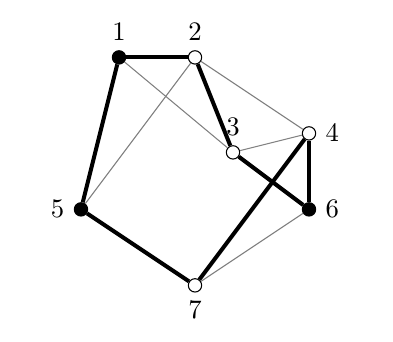
\includegraphics[width=0.4\textwidth]{ejemplo_0.png}
    \caption{Una instancia con B = \textbraceleft 1, 5, 6\textbraceright, W = \textbraceleft 2, 3, 4, 7\textbraceright, y una solución factible indicada por las aristas gruesas para Q = 2 y L = 3. La solución es óptima, por ejemplo, cuando el costo y la distancia de cada arista es 1 para todas las contenidas en la solución, y 2 para el resto.}
    \label{fig:ejemplo_0}
\end{figure}

Entre las aplicaciones de este problema están las operaciones aéreas de trayectos cortos. En este caso los vértices negros pueden representar estaciones de mantenimiento que los aviones tienen que visitar después de Q + 1 tramos como máximo, o después de haber recorrido una distancia máxima de L.


\section{Branch and Cut}
Branch and cut es un método de optimización combinatoria para resolver problemas de programación lineal entera, en particular, es el método utilizado en el paper estudiado.\\
La idea detrás de este método, es usar una combinación del método de \textit{planos de corte} con algoritmos de \textit{branch-and-bound}. Estos métodos, funcionan resolviendo una secuencia de \textit{relajaciones lineales} del problema en enteros, es decir, ignorar temporalmente la restricción de tener variables enteras.\\
Por ejemplo, en programa entero 0-1, las restricciones tienen la pinta:
$$x_i \in \{0,1\}$$
La relajación lineal del problema usa las siguientes restricciones:
$$0 \leq x_i \leq 1$$
La técnica de relajación convierte un problema de optimización NP-Hard en un problema relacionado que puede ser resuelto en tiempo polinomial. La solución obtenida con la relajación puede ser usada para ganar información sobre el problema original. 
\subsection{Planos de corte}
La idea detrás del método de planos de corte es ir agregando restricciones a un programa lineal hasta que la solución óptima factible tenga valores enteros. Por supuesto, teniendo cuidado con las restricciones que se añaden para que no cambie el problema.\\
Llamaremos a las resticciones que se añaden, \textit{cortes}. Un corte relativo a una solución fraccional actual, debe satisfacer las siguientes condiciones,
\begin{itemize}
  \item Toda solución entera factible debe ser factible con el corte
  \item La solución fraccionaria actual no debe ser factible con el corte
\end{itemize}

En la figura \ref{fig:ejemplo_cut} se puede ver un ejemplo gráfico de un corte. El círculo rojo representa la solución óptima fraccionaria encontrada. Los círculos negros son las soluciones enteras y la línea roja representa un corte que cumple con ambos requisitos, acotando nuestro espacio de soluciones factibles.\\
\begin{figure}[H]
  \centering
  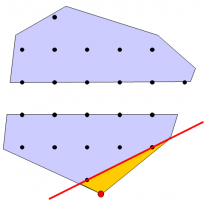
\includegraphics[width=0.4\textwidth]{ejemplo_cut.png}
  \caption{La linea roja representa un corte posible en una instancia.}
  \label{fig:ejemplo_cut}
\end{figure}

Hay dos formas de generar cortes. La primera, los cortes de Gomory genera cortes para cualquier problema de programación lineal. Esta tiene la venteja de "resolver" cualquier problema, pero la desventaja de que puede ser muy lento. El segundo enfoque, consiste en utilizar la estructura del problema que se quiere resolver para conseguir buenos cortes. De esta forma se pueden conseguir resultados muy buenos pero con la desventaja de tener que hacer un análisis para cada problema por separado.\\
\subsection{Branch and Bound}


\section{Modelos}


\[
\arraycolsep=1pt\def\arraystretch{1.5}
\begin{array}{cccc}
	\min & \sum_{e \in E} c_{e} x_{e} & & (1) \\
	\text { tal que } & \quad x(\delta(i))=2 & \forall i \in V & (2) \\
	& x(E(S)) \geq 2 & \forall S \subseteq V \backslash\{1\},\ S \neq \emptyset & (3) \\
	& \left\{e \in E : x_{e}=1\right\} & \text { satisface la restricción de salto para el camino después de cada } k \in B & (4) \\
	& \left\{e \in E : x_{e}=1\right\} & \text { satisface la restricción de distancia para el camino después de cada } k \in B & (5) \\
	& \mathbf{x} \in\{0,1\}^{|E|} & & (6) 
\end{array}
\]

\section{Modelo de porción del camino}

\[
\arraycolsep=20pt\def\arraystretch{1.5}
\begin{array}{ccc}
	x^{k}\left(\delta^{+}(k)\right)=1 & \forall k \in B & (7) \\
	\sum_{j \in B \backslash\{k\}} x^{j}\left(\delta^{-}(k)\right)=1 & \forall k \in B & (8) \\
	x^{k}\left(\delta^{-}(i)\right)=x^{k}\left(\delta^{+}(i)\right) & \forall k \in B,\ \forall i \in W & (9) \\
	\sum_{k \in B} x_{i j}^{k}+x_{j i}^{k}=x_{e} & \forall e=\{i, j\} \in E & (10)
\end{array}
\]

\section{Formulaciones dependientes de la posición}

\subsection{Formulación pura}

\subsection{Formulación de una porción del camino}

(Modelos traducidos así nomás. Hay que mejorar seguro este)

\subsection{Modelo 2-dimensional}

\section{Modelos alternativos dependientes del tiempo}

\section{Comparaciones teóricas}

\subsection{Pre-procesamiento}

\subsection{Algoritmo de plano de corte}

\subsection{Heurísticas}

\section{Resultados empíricos}

(Por ahí habría que mejorar este título)

\subsection{Instancias}

\subsection{Relajaciones}

\subsection{Análisis de los resultados}

\pagebreak

\begin{thebibliography}{9}

\bibitem{main}
L. Gouveia, M. Leitner y M. Ruthmair, “Extended formulations and branch-and-cut algorithms for the Black-and-White Traveling Salesman Problem". European Journal of Operational Research, 262-3, 908-928. 2017.
G. Cornuéjols, M. Trick y M. Saltzman, "A tutorial on integer programming". CMU Technical Report (1995).
G. Pataki, "Teaching integer programming formulations using the traveling salesman problem". SIAM Review 45-1 (2003) 116-123.
John E., Mitchell (2002). "Branch-and-Cut Algorithms for Combinatorial Optimization Problems"
\end{thebibliography}

\end{document}